
%!TEX ROOT=ctutest.tex
\chapter{Realizace FW}
\section{Rozpoznání frekvence externího krystalu HSE}
Pro chod mikrokonroléru je zapotřebí zdroj hodinového signálu pro generování systémových hodin(System Core clock) dále jen SYSCLK. Jako základní varianta zdroje hodinového signálu se používá interní vysoko-rychlostní oscilátor(HSI), jehož výstupní frekvence ve srovnání s externími zdroji hodinového signálu vykazuje řádově vyšší nepřesnost a vyšší závislost na změnách teplot viz srovnávací tabulka\ref{tab:HSE}.Tento rozdíl je pak obzvlášť podstatný při realizaci funkce osciloskopu v režimu vzorkování v ekvivalentním čase(ETS), kde dochází k výraznému zkreslení měřeného signálu viz obrázek \ref{fig:signaldistortionhsi}. Na tomto obrázku je zobrazen zkreslený záznam signálu s G431 využívajícím HSI jako zdroj hodinového signálu a druhá stopa je měřena osciloskopem Rigol DS1052E jehož přesnost vzorkovací frekvence je $\pm0.005\%$ \cite{ScopeRigol}. Z obrázku je zřejmá vhodnost použití zdroje hodinového signálu s vyšší přesností než vykazuje HSI.

\begin{figure}[H]
	\centering
	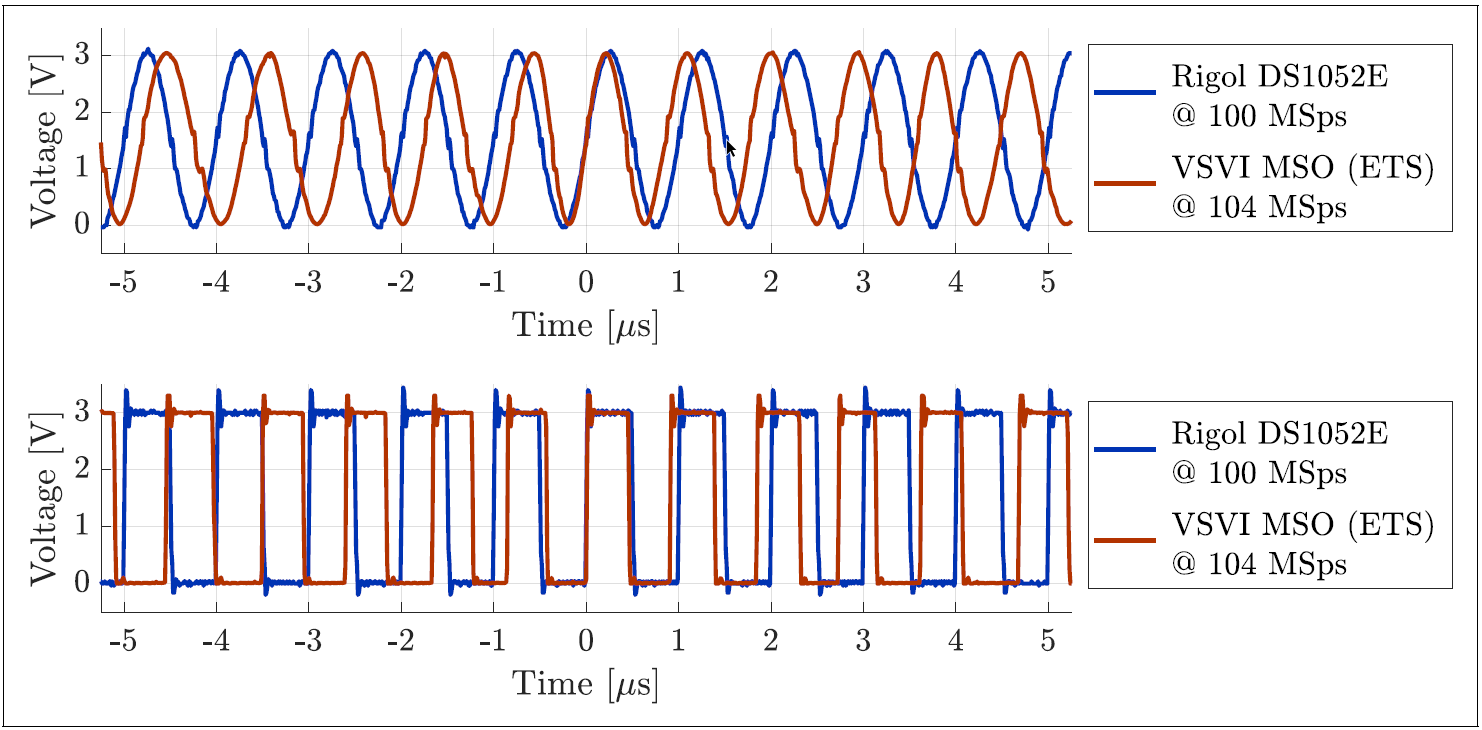
\includegraphics[width=0.7\linewidth]{Figs/Graphs/SignalDistortion_HSI}
	\caption{Zkreslení průběhu měřeného signálu v důsledku nestability HSI převzato z \cite{DujavaDIP}}
	\label{fig:signaldistortionhsi}
\end{figure}

Jako zdroj vysokorychlostního externě získaného hodinové signálu(HSE) lze buď využít krystalu buzeného pomocí MCU(HSE crystal) nebo jiného externího zdroje signálu(HSE bypass). Případný externí signál musí pak splňovat nějaké podmínky a to například pro STM32G431 musí být v rozsahu 4-48MHz a mít střídu 40-60\%. Ve výuce laboratorních měření na katedře měření jsou k dispozici krystaly různých výstupních frekvencí převážně pak 8 MHz, 12MHz a 16MHz.Pro  účely co nejflexibilnějšího laboratorního přístroje se zdálo účelné naprogramovat firmware pro použití s různými takovýmito oscilátory.Tedy aby funkce FW nebyla závislá na přítomnosti krystalu ani jeho výstupní frekvenci. Toho bylo docíleno změřením výstupní frekvence oscilátoru a nastavení výsledné frekvence systémových hodin pomocí interního obvodu fázového závěsu(PLL), tak aby výsledná frekvence SYSCLK nebyla na použitém krystalu závislá.

\begin{table}[H]
	\begin{tabular}{l|rr}
		& $\Delta$ f & $\Delta$ \\ \hline
		STM32G431 HSI 16 MHz     & $\pm$ 1\%       & $\pm$1\%      \\ \hline
		Adafruit krystal 16 MHz & $\pm$0.003\%   & $\pm$0.005\% 
	\end{tabular}
	\caption{}
	\label{tab:HSE}
\end{table}

\subsection{Měření frekvence HSE}
Existují různé způsoby měření frekvence externího hodinového signálu, ale jako nejčúčelnější se v tomto případě zdálo použítí čítače v režimu "Input capture"(IC) a měřit délku periody externího signálu. Na rodině mikrokontrolérů STM32G4 mají čítače TIM16 a TIM17 možnost interně přivést HSE již se sníženou frekvencí. Frekvence HSE je totiž ještě před přivedením na vstup čítače zpracovaná obvodem, který frekvenci 32krát sníží. Pro tento vstup čítače se sníženou frekvencí se pak používá označení HSE32 jako je vidět na obrázku \ref{fig:tim16inputs} z dokumentace.

% TODO: \usepackage{graphicx} required
\begin{figure}[H]
	\centering
	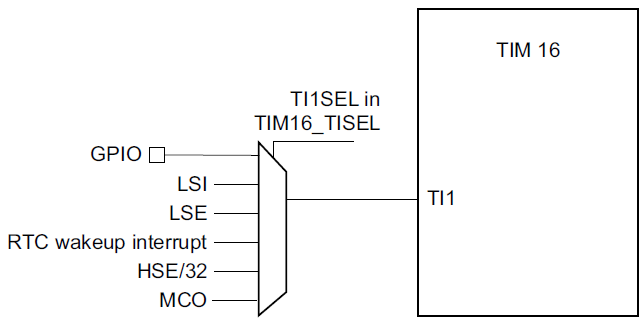
\includegraphics[width=0.7\linewidth]{Figs/Documentation/TIM16_Inputs}
	\caption[Vstupy čítače TIM16]{Vstupy dostupné na kanálu číslo 1 čítače TIM16. Převzato z\cite{refG4}}
	\label{fig:tim16inputs}
\end{figure}

Měření periody signálu HSE32 probíhá potom tak, že měříme počet cyklů čítače mezi jednotlivými náběžnými hranami nebo sestupnými hranami. Tento počet cyklů nám pak určuje poměr mezi frekvencí externího hodinového signálu na vstupu $	f_{\text{IN}}$ a hodinového signálu, který pro svůj chod využívá periferie čítače $	f_{\text{TIM}}$. Pro správné měření je tedy podstatné, aby interní hodinový signál čítače byl výrazně vyšší než frekvence na měřeném vstupu. Pro získání přesnějšího odhadu vstupní frekvence můžeme zaznamenat více hodnot hodnot po sobě a ty poté zprůměrovat. Frekvence vstupu je poté rovna:
\begin{equation}
	f_{\text{IN}}=\frac{f_{\text{TIM}}}{N_\text{p}}
\end{equation}
Pro určení frekvence HSE pak ještě musíme získanou hodnotu vynásobit 32:
\begin{equation}
	f_{\text{HSE}}=32 \cdot f_{\text{IN}}
\end{equation}
\subsection{Využití PLL}
Obvod PLL je další z možných zdrojů hodinového signálů systémových hodin, který má navíc programovatelné dělení a násobení vstupní frekvence. Jako vstup pak lze použít HSI nebo HSE ve stanovené rozsahu. Například 2.66-16MHz  pro stm32G431\cite{dataG431}. Dle obrázku \ref{fig:plldiagram} lze vidět jak vstupní hodinový signál vstupujícího do PLL bloku  nejdříve prochází přes děličku signálu M, dále se hodinový signál násobí N a tento signál jde pak na 3 různé výstupy s vlastními děličkami. Dále v kapitole o ADC ukazuji výhodu této možnosti více výstupů z obvodu PLL díky které vstupní hodiny ADC nemusí být závislé na frekvenci systémových hodin. 

\begin{figure}[H]
	\centering
	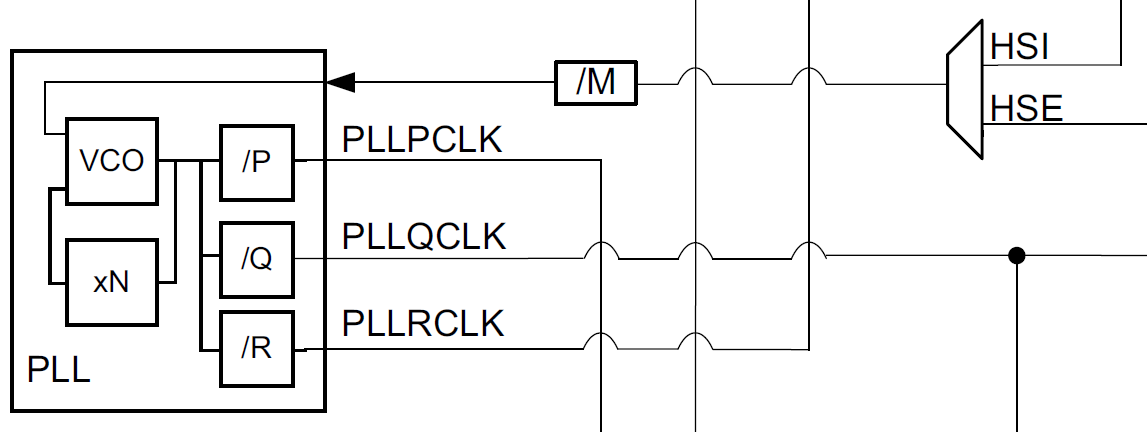
\includegraphics[width=0.6\linewidth]{Figs/Documentation/PLL_Diagram}
	\caption{Vyobrazení interního PLL bloku. Převzato z}
	\label{fig:plldiagram}
\end{figure}    

\subsection{Změna zdroje hodinového signálu systémových hodin}
Na obrázku \ref{fig:hsekonfigurace} je popsaný postup změny zdroje SYSCLK. Při změně vstupního signálu PLL nelze PLL používat, tedy je nejdříve zapotřebí přepnout systémové hodiny na interní oscilátor 16MHz. Dle doporučení v \cite{refG4} je při velkých rozdílech frekvencí mezi výstupem PLL(SYSCLK>80MHz) zapotřebí přidat mezikrok s využitím AHB předděličky hodinového signálu systémových hodin. hodnota předděličky se nastavuje RCC\_CFGR registru. Díky tomu například ve svém programu zmenším frekvenci systémových na polovinu tedy 78 MHz a pak až nastavuji jako zdroj HSI146. Doporučená doba setrvání v tomto mezikroku je alespoň $1\mu$s. V mém řešení program čeká 1ms s využitím připravených funkcí obsahujícím čekání v jednotkách ms.


\begin{figure}[H]
	\centering
	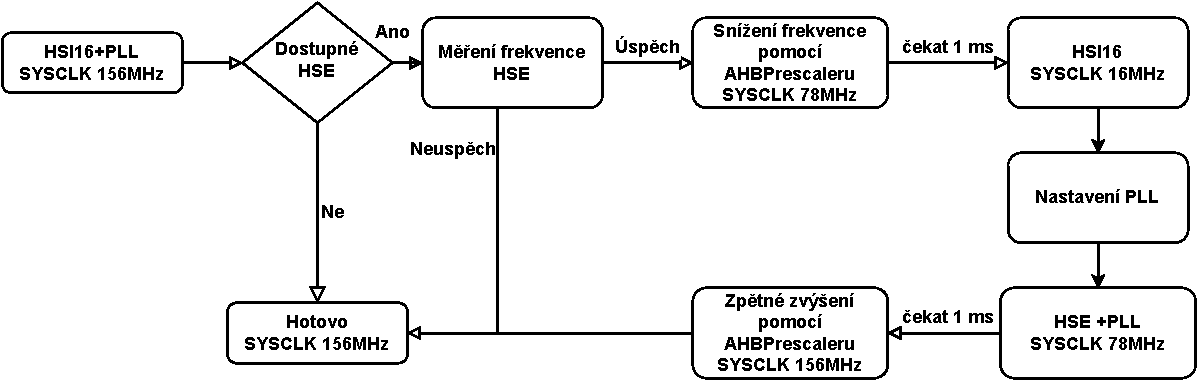
\includegraphics[width=1\linewidth]{Figs/Documentation/HSE_Konfigurace}
	\caption{Postup změny zdroje hodinového signálu}
	\label{fig:hsekonfigurace}
\end{figure}
\section{Struktura FW}
\subsection{Využití LL driverů}
\subsection{Core coupled memory CCM SRAM}
\section{Realizace funkce Voltmetru}
\subsection{Nejistota měření}
\section{Realizace měření frekvence}
\subsection{Nejistota měření}
\section{Realizace funkce generátoru}
\subsection{Generování signálu}
\subsubsection{Využití CORDIC}    
\subsection{Generování šumu}
\section{Realizace osciloskopu}
\subsection{Mody měření}
\section{Logický analyzátor}
\chapter{Ověření funkčnosti}



